\documentclass{article}
\usepackage{physics}
\usepackage{graphicx}
\usepackage{caption}
\usepackage{amsmath}
\usepackage{bm}
\usepackage{framed}
\usepackage{authblk}
\usepackage{empheq}
\usepackage{amsfonts}
\usepackage{esint}
\usepackage[makeroom]{cancel}
\usepackage{dsfont}
\usepackage{centernot}
\usepackage{mathtools}
\usepackage{subcaption}
\usepackage{bigints}
\usepackage{amsthm}
\theoremstyle{definition}
\newtheorem{lemma}{Lemma}
\newtheorem{defn}{Definition}[section]
\newtheorem{prop}{Proposition}[section]
\newtheorem{rmk}{Remark}[section]
\newtheorem{thm}{Theorem}[section]
\newtheorem{exmp}{Example}[section]
\newtheorem{prob}{Problem}[section]
\newtheorem{sln}{Solution}[section]
\newtheorem*{prob*}{Problem}
\newtheorem{exer}{Exercise}[section]
\newtheorem*{exer*}{Exercise}
\newtheorem*{sln*}{Solution}
\usepackage{empheq}
\usepackage{tensor}
\usepackage{xcolor}
%\definecolor{colby}{rgb}{0.0, 0.0, 0.5}
\definecolor{MIT}{RGB}{163, 31, 52}
\usepackage[pdftex]{hyperref}
%\hypersetup{colorlinks,urlcolor=colby}
\hypersetup{colorlinks,linkcolor={MIT},citecolor={MIT},urlcolor={MIT}}  
\usepackage[left=1in,right=1in,top=1in,bottom=1in]{geometry}

\usepackage{newpxtext,newpxmath}
\newcommand*\widefbox[1]{\fbox{\hspace{2em}#1\hspace{2em}}}

\newcommand{\p}{\partial}
\newcommand{\R}{\mathbb{R}}
\newcommand{\C}{\mathbb{C}}
\newcommand{\lag}{\mathcal{L}}
\newcommand{\nn}{\nonumber}
\newcommand{\ham}{\mathcal{H}}
\newcommand{\M}{\mathcal{M}}
\newcommand{\I}{\mathcal{I}}
\newcommand{\K}{\mathcal{K}}
\newcommand{\F}{\mathcal{F}}
\newcommand{\w}{\omega}
\newcommand{\lam}{\lambda}
\newcommand{\al}{\alpha}
\newcommand{\be}{\beta}
\newcommand{\x}{\xi}

\newcommand{\G}{\mathcal{G}}

\newcommand{\f}[2]{\frac{#1}{#2}}

\newcommand{\ift}{\infty}

\newcommand{\lp}{\left(}
\newcommand{\rp}{\right)}

\newcommand{\lb}{\left[}
\newcommand{\rb}{\right]}

\newcommand{\lc}{\left\{}
\newcommand{\rc}{\right\}}


\newcommand{\V}{\mathbf{V}}
\newcommand{\U}{\mathcal{U}}
\newcommand{\Id}{\mathcal{I}}
\newcommand{\D}{\mathcal{D}}
\newcommand{\Z}{\mathcal{Z}}

%\setcounter{chapter}{-1}


\usepackage{enumitem}



\usepackage{listings}
\captionsetup[lstlisting]{margin=0cm,format=hang,font=small,format=plain,labelfont={bf,up},textfont={it}}
\renewcommand*{\lstlistingname}{Code \textcolor{violet}{\textsl{Mathematica}}}
\definecolor{gris245}{RGB}{245,245,245}
\definecolor{olive}{RGB}{50,140,50}
\definecolor{brun}{RGB}{175,100,80}

%\hypersetup{colorlinks,urlcolor=colby}
\lstset{
	tabsize=4,
	frame=single,
	language=mathematica,
	basicstyle=\scriptsize\ttfamily,
	keywordstyle=\color{black},
	backgroundcolor=\color{gris245},
	commentstyle=\color{gray},
	showstringspaces=false,
	emph={
		r1,
		r2,
		epsilon,epsilon_,
		Newton,Newton_
	},emphstyle={\color{olive}},
	emph={[2]
		L,
		CouleurCourbe,
		PotentielEffectif,
		IdCourbe,
		Courbe
	},emphstyle={[2]\color{blue}},
	emph={[3]r,r_,n,n_},emphstyle={[3]\color{magenta}}
}


\begin{document}
\begin{framed}
\noindent Name: \textbf{Huan Q. Bui}\\
Course: \textbf{8.422 - AMO II}\\
Problem set: \textbf{\#5}\\
Due: Friday, Mar 17, 2022\\
Collaborators: Minh-Thi Nguyen 
\end{framed}
	


\noindent \textbf{1. Better Phase Measurement with Squeezed Vacuum.}\\

\noindent One application of squeezed light is to measure phase shifts with better precision than can be
achieved with the same number of photons in a coherent state.  In this problem, we employ a
Mach-Zehnder interferometer with coherent and squeezed input states. This interferometer uses two 50/50 beamsplitters and has a phase shift in one path of $\phi$ and has output ports of $b_\text{out}$ and $a_\text{out}$. 

\begin{figure*}[!htb]
\centering
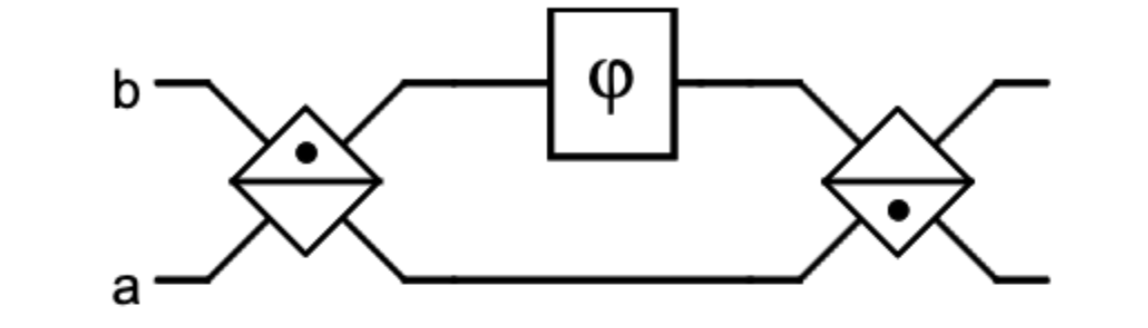
\includegraphics[width=0.4\textwidth]{figures/BS.png}
\end{figure*}



\begin{enumerate}[label=(\alph*)]

\item Suppose the input on port $a$ is a coherent state $\ket{\al}$ and the input on port $b$ is the vacuum state $\ket{0}$. Here we calculate the output signal $\langle M \rangle = \langle b_\text{out}^\dagger b_\text{out} - a_\text{out} ^\dagger a_\text{out} \rangle$, its variance $\langle  \Delta M^2 \rangle = \langle \Delta (b_\text{output}^\dagger b_\text{output} - a_\text{output}^\dagger a_\text{output})^2$, and the signal-to-noise ratio $\langle M \rangle / \sqrt{\langle \Delta M^2 \rangle}$.\\

Let's first compute the output ports in terms of the input ports. After the first beamsplitter, we have 
\begin{align*}
b_1 = BbB^\dagger  = \f{b-a}{\sqrt{2}} \quad\quad \text{and} \quad\quad a_1 = BaB^\dagger = \f{b+a}{\sqrt{2}}.
\end{align*}
Remembering that the beamsplitter with the dot facing up is $B$, we calculate the output after it:
\begin{align*}
B\ket{\al}_a \ket{0}_b = e^{-\abs{\al}^2/2} B e^{\al a^\dagger } B^\dagger \ket{0}_a \ket{0}_b = 
e^{-\abs{\al}^2/2}\exp\lp \al \f{a^\dagger + b^\dagger }{\sqrt{2}} \rp \ket{0}\ket{0} = 
\ket{\f{\al}{\sqrt{2}} }_{a_1} \ket{ \f{\al}{\sqrt{2}}}_{b_1}.
\end{align*}
After the phase shift in the $b$ mode we have
\begin{align*}
\ket{\f{\al}{\sqrt{2}} }_{a_1} \ket{ \f{\al}{\sqrt{2}}}_{b_1} \to \
 \ket{\f{\al}{\sqrt{2}} }_{a_1} \ket{ \f{\al e^{i\varphi}}{\sqrt{2}}}_{b_1}.
\end{align*}
Finally, we apply $B^\dagger$ to this state: 
\begin{align*}
B^\dagger  \ket{\f{\al}{\sqrt{2}} }_{a_1} \ket{ \f{\al e^{i\varphi}}{\sqrt{2}}}_{b_1} 
&= e^{-\abs{\al}^2/2} B^\dagger e^{\al a^\dagger  /\sqrt{2}} e^{\al e^{i\varphi} b^\dagger  /\sqrt{2}  } BB^\dagger \ket{0} \ket{0} \\
&= e^{-\abs{\al}^2/2} \exp\lp \f{\al}{2}(  a^\dagger - b^\dagger)  + \f{\al e^{i\varphi}}{2}(a^\dagger + b^\dagger ) \rp  \ket{0} \ket{0}\\
&= e^{-\abs{\al}^2/2} \exp\lp a^\dagger \f{\al(1 + e^{i\varphi})}{2} + b^\dagger \f{\al(-1 + e^{i\varphi})}{2} \rp \ket{0} \ket{0}\\
&= \ket{\f{\al(1+e^{i\varphi})}{2}}_{a_\text{out}} \ket{\f{\al(-1+e^{i\varphi})}{2}}_{b_\text{out}}.
\end{align*}
With this we can compute the signal:
\begin{align*}
\langle M \rangle = \langle b_\text{out}^\dagger b_\text{out} - a_\text{out}^\dagger a_\text{out} \rangle 
= \langle b_\text{out}^\dagger b_\text{out} \rangle - \langle a_\text{out}^\dagger a_\text{out} \rangle 
= \f{\abs{\al}^2}{4}\abs{-1+e^{i\varphi}}^2  - \f{\abs{\al}^2}{4} \abs{1+e^{i\varphi}}^2 
= \boxed{- \abs{\al}^2 \cos\varphi }
\end{align*}
Next we compute the variance in the signal:
\begin{align*}
\langle \Delta M^2 \rangle 
&= \langle M^2\rangle - \langle M \rangle^2\\ 
&= \langle (b_\text{out}^\dagger b_\text{out} - a_\text{out}^\dagger a_\text{out})^2 \rangle - \abs{\al}^4\cos^2\varphi \\ 
&= \langle  b_\text{out}^\dagger b_\text{out} b_\text{out}^\dagger b_\text{out} + 
a_\text{out}^\dagger a_\text{out}a_\text{out}^\dagger a_\text{out}  
- 2 b_\text{out}^\dagger b_\text{out}a_\text{out}^\dagger a_\text{out} \rangle - \abs{\al}^4 \cos^2\varphi\\ 
&= \langle n^2_{b,\text{out}} \rangle + \langle n^2_{a,\text{out}} \rangle 
-2 \langle n_{b,\text{out}} \rangle  \langle n_{a,\text{out}} \rangle - \abs{\al}^4 \cos^2 \varphi \\ 
&= \abs{\f{\al(-1 + e^{i\varphi})}{2}}^4 + \abs{\f{\al(-1 + e^{i\varphi})}{2}}^2 
+ \abs{\f{\al(1+ e^{i\varphi})}{2}}^4 + \abs{\f{\al(1+ e^{i\varphi})}{2}}^2 \\
&\quad - 2 \abs{\f{\al(-1 + e^{i\varphi})}{2}}^2 \abs{ \f{\al(1 + e^{i\varphi})}{2}}^2 
- \abs{\al}^4\cos^2\varphi\\
&= \f{\abs{\al}^4}{16}( 16 \cos^2\varphi  ) - \abs{\al}^4 \cos^2\varphi
+ \f{4\abs{\al}^2}{4}\\
&= \boxed{\abs{\al}^2}
\end{align*}
With these, the sign-to-noise ratio in the signal is 
\begin{align*}
\text{SNR} = \abs{ \f{\langle M\rangle}{\sqrt{\langle \Delta M^2 \rangle}} }= \f{\abs{\al}^2 \abs{ \cos\varphi}}{\abs{\al}} = \boxed{\abs{\al \cos\varphi}}
\end{align*}
\textcolor{purple}{There could be a point of confusion here as to which states we want to use to evaluate the expectation values. The approach above uses the output states, since the operators $b_\text{out}., b_\text{out}^\dagger, a_\text{out}, a_\text{out}^\dagger$ act on the output states like $b^\dagger, b, a^\dagger, a$. So that is clear. This means the expectation value should have written, most explicitly, as $_\text{out} \langle (\text{-out-}) \rangle_\text{out}$. Otherwise, one can interpret it as evaluating the expectation values using the input states, which one can do, but has to be careful since the operators $b_\text{out}^\dagger, b, a_\text{out}^\dagger, a$ must be transformed into the forms involving $b^\dagger, b, a^\dagger, a$ using the beamsplitter and phase operators. But okay, life goes on.}



\item The minimal detectable phase is the phase $\phi_\text{min}$ for which $\text{SNR} = 1$. Assuming we have a strong coherent state then $\cos \varphi$ is small. This means we want to expand $\cos \varphi$ near $\pi/2$.
\begin{align*}
1 = \abs{\al} \cos\varphi_\text{min} \approx  \pm \abs{\al} \lp \varphi_\text{min} - \f{\pi}{2}  \rp \implies \varphi_\text{min} \approx \boxed{ \pm \f{1}{\abs{\al}} + \f{\pi}{2}}
\end{align*}
If we want the answer for minimal detectable phase \textit{difference} which is what we ultimately care about, then the answer is $\boxed{\varphi_\text{min} = 1/\abs{\al}}$.

\item Now we repeat the calculation but with the squeezed vacuum $S(z) \ket{0}$ entering port $b$ instead, where $z = re^{i\phi}$. Instead of finding what the states are explicitly after each optical component like we did last time (as this will be very complicated), let us write down the full expectation value and simplify things from top level:
\begin{align*}
\langle M \rangle = \langle b_\text{out}^\dagger b_\text{out} - a_\text{out}^\dagger a_\text{out} \rangle 
&= \bra{0_{r,b} \al_a} B^\dagger \Phi^\dagger B   (b^\dagger b - a^\dagger a) B^\dagger \Phi B  \ket{0_{r,b} \al_a}\\
&= \bra{0_{r,b} \al_a} B^\dagger e^{-i \hat{n}_b \varphi} B   (b^\dagger b - a^\dagger a) B^\dagger e^{i \hat{n}_b \varphi} B  \ket{0_{r,b} \al_a}.
\end{align*}
Now we slowly unpack:
\begin{align*}
B(b^\dagger b - a^\dagger a) B^\dagger 
= \f{1}{2}\lb (b^\dagger - a^\dagger)(b-a) - (b^\dagger + a^\dagger)(b+a) \rb = -ab^\dagger - a^\dagger b.
\end{align*}
Next, the phase operator acts on $b$ as $\Phi^\dagger b^\dagger \Phi = b^\dagger e^{i\varphi}$, which we obtain from looking at how the phase operator acts on a coherent state. With this, 
\begin{align*}
e^{-i \hat{n}_b \varphi} (-ab^\dagger - a^\dagger b) e^{i \hat{n}_b \varphi} = -a e^{-i b^\dagger b \varphi}  b^\dagger e^{i b^\dagger b \varphi} - a^\dagger e^{-i b^\dagger b \varphi} b e^{i b^\dagger b \varphi} = 
-a b^\dagger e^{i\varphi} - a^\dagger b e^{-i\varphi}.
\end{align*}
Finally, we do the last beamsplitter transformation. We make use of $[a,a^\dagger] = [b,b^\dagger] = 1$ to find:
\begin{align*}
B^\dagger (-a b^\dagger e^{i\varphi} - a^\dagger b e^{-i\varphi}) B 
&= -\f{e^{i\varphi}}{2}(a-b) (b^\dagger + a^\dagger) -\f{e^{-i\varphi}}{2}(a^\dagger - b^\dagger) (b + a) \\
&= -\f{e^{i\varphi}}{2}(aa^\dagger +ab^\dagger - a^\dagger b - bb^\dagger) - \f{e^{-i\varphi}}{2}(a^\dagger a + a^\dagger b - ab^\dagger - b^\dagger b)\\
&= -\f{e^{i\varphi}}{2}(a^\dagger a +ab^\dagger - a^\dagger b - b^\dagger b) - \f{e^{-i\varphi}}{2}(a^\dagger a + a^\dagger b - ab^\dagger - b^\dagger b) \\
&=
-(\cos\varphi) a^\dagger a  
+ 
(i\sin\varphi) a^\dagger b 
- 
(i\sin\varphi) ab^\dagger 
+ 
(\cos\varphi) b^\dagger b.
\end{align*}
Thus,
\begin{align*}
\langle M \rangle = -\abs{\al}^2 \cos\varphi + \bra{0_{z,b}} b^\dagger b \ket{0_{z,b}} \cos \varphi 
= 
\boxed{\cos\varphi \lp \sinh^2 r - \abs{\al}^2 \rp}
\end{align*}
Without doing much more, we can already answer that \boxed{\textbf{YES}}, squeezing changes the average photon number in the device. \\


\noindent Next we compute $\langle \Delta M^2 \rangle = \langle M^2 \rangle - \langle M \rangle^2$. First, 
\begin{align*}
\langle M^2 \rangle 
= \langle (b_\text{out}^\dagger b_\text{out} - a_\text{out}^\dagger a_\text{out})^2 \rangle 
&= \bra{0_{r,b} \al_a} B^\dagger \Phi^\dagger B   (b^\dagger b - a^\dagger a)^2 B^\dagger \Phi B  \ket{0_{r,b} \al_a}\\
&= \bra{0_{r,b} \al_a} B^\dagger e^{-i \hat{n}_b \varphi} B   (b^\dagger b - a^\dagger a)^2 B^\dagger e^{i \hat{n}_b \varphi} B  \ket{0_{r,b} \al_a}.
\end{align*}
We once again slowly unpack:
\begin{align*}
B   (b^\dagger b - a^\dagger a)^2 B^\dagger = [B   (b^\dagger b - a^\dagger a) B^\dagger]^2  = (ab^\dagger + a^\dagger b)^2 
\end{align*}
Now we let the phase transformation act:
\begin{align*}
e^{-i \hat{n}_b \varphi} (ab^\dagger + a^\dagger b)^2 e^{i \hat{n}_b \varphi} = [ e^{-i \hat{n}_b \varphi} (ab^\dagger + a^\dagger b) e^{i \hat{n}_b \varphi}   ]^2 = (a b^\dagger e^{i\varphi} + a^\dagger b e^{-i\varphi})^2
\end{align*}
The final beamsplitter transformation gives 
\begin{align*}
B^\dagger (a b^\dagger e^{i\varphi} + a^\dagger b e^{-i\varphi})^2 B 
&= [ -(\cos\varphi) a^\dagger a  
+ 
(i\sin\varphi) a^\dagger b 
- 
(i\sin\varphi) ab^\dagger 
+ 
(\cos\varphi) b^\dagger b ]^2 \\
&= [\cos\varphi (b^\dagger b - a^\dagger a) + i\sin\varphi (a^\dagger b - ab^\dagger )   ]^2 \\
&= \cos^2\varphi (b^\dagger b - a^\dagger a)^2 - \sin^2\varphi ( a^\dagger b - ab^\dagger )^2 \\
&\quad + i\cos\varphi\sin\varphi (b^\dagger b - a^\dagger a)( a^\dagger b -ab^\dagger) 
+ i\cos\varphi\sin\varphi (a^\dagger b - ab^\dagger)(b^\dagger b - a^\dagger a).
\end{align*}
What, then, is $\langle M^2 \rangle$? We first notice that all terms with $i\sin\varphi\cos\varphi$ do not contribute since there is always an odd number of $a$ or $a^\dagger$. With this fact, we can calculate:
\begin{align*}
\langle M^2 \rangle 
&= \cos^2\varphi \langle (b^\dagger b - a^\dagger a )^2 \rangle - \sin^2 \varphi \langle (a^\dagger b - ab^\dagger )^2 \rangle \\ 
&= \cos^2 \varphi \langle  (b^\dagger b)^2 - 2 b^\dagger b a^\dagger a + (a^\dagger a)^2  \rangle - \sin^2 \varphi \langle  a^\dagger a^\dagger bb - a^\dagger a bb^\dagger - aa^\dagger b^\dagger b + aab^\dagger b^\dagger  \rangle \\
&= \cos^2 \varphi \langle  (b^\dagger b)^2 - 2 b^\dagger b a^\dagger a + (a^\dagger a)^2  \rangle 
- \sin^2 \varphi \langle  a^\dagger a^\dagger bb - a^\dagger a (1+b^\dagger b) - (1+a^\dagger a) b^\dagger b + aab^\dagger b^\dagger  \rangle.
\end{align*}
Now we have to evaluate $\langle bb \rangle$ and $\langle b^\dagger b^\dagger \rangle$. Using 
\begin{align*}
\begin{pmatrix}
S^\dagger(z) b S(z) \\ S^\dagger(z) b^\dagger S(z)
\end{pmatrix}
= 
\begin{pmatrix}
\cosh r & -e^{i\phi} \sinh r \\ -e^{-i\phi}\sinh r & \cosh r 
\end{pmatrix}
\begin{pmatrix}
b \\ b^\dagger 
\end{pmatrix}
\end{align*}
we find 
\begin{align*}
\bra{0_{z,b}}  bb    \ket{0_{z,b}}  = \bra{0}  ( b\cosh r - b^\dagger e^{i\phi} \sinh r)^2  \ket{0} = -e^{i\phi}\cosh r \sinh r
\end{align*}
and 
\begin{align*}
\bra{0_{z,b}}  b^\dagger b^\dagger    \ket{0_{z,b}}  = \bra{0}  ( b^\dagger \cosh r - b e^{-i\phi} \sinh r)^2  \ket{0} = -e^{-i\phi}\cosh r \sinh r.
\end{align*}
Finally, we have to evaluate $\langle (b^\dagger b)^2 \rangle$:
\begin{align*}
\langle (b^\dagger b)^2 \rangle 
&= \bra{0} [(b^\dagger \cosh r - b e^{-i\phi} \sinh r)(b\cosh r - b^\dagger e^{i\phi}\sinh r)]^2   \ket{0}.
\end{align*}
Let's expand the inside:
\begin{align*}
 &[(b^\dagger \cosh r - b e^{-i\phi} \sinh r)(b\cosh r - b^\dagger e^{i\phi}\sinh r)]^2 \\
 =\,\,& [ b^\dagger b \cosh^2 r  -b^\dagger b^\dagger e^{i\phi}\sinh r\cosh r - bb e^{-i\phi}\sinh r \cosh r + bb^\dagger \sinh^2 r]^2.
\end{align*}
We need to evaluate the expectation value of the term above with respect to the vacuum. The only terms that contribute are $bbb^\dagger b^\dagger$ and $bb^\dagger b b^\dagger$:
\begin{align*}
\bra{0_{z,b}} (b^\dagger b )^2 \ket{0_{z,b}}
&= \sinh^2 r \cosh^2 r   \bra{0} bbb^\dagger b^\dagger  \ket{0}  + \sinh^4 r \bra{0} bb^\dagger b b^\dagger \ket{0} \\ 
&= 2 \sinh^2 r \cosh^2 r + \sinh^4 r.
\end{align*}
Putting everything together we find 
\begin{align*}
\langle M^2 \rangle 
&= \cos^2 \varphi 
\lb 2 \sinh^2 r \cosh^2 r + \sinh^4 r - 2 \abs{\al}^2\sinh^2 r + \abs{\al}^4 + \abs{\al}^2  \rb \\ 
&\quad - \sin^2 \varphi \lb -{\al^*}^2 e^{i\phi} \cosh r \sinh r - \abs{\al}^2(1 + \sinh^2 r) - (1+\abs{\al}^2)\sinh^2 r 
- \al^2  e^{-i\phi} \cosh r \sinh r    \rb
\end{align*}
And so the variance in the signal is 
\begin{align*}
\langle \Delta M^2 \rangle 
&= \langle M^2 \rangle - \langle M\rangle^2 \\
&= \cos^2 \varphi 
\lb 2 \sinh^2 r \cosh^2 r + \abs{\al}^2  \rb \\ 
&\quad - \sin^2 \varphi \lb -{\al^*}^2 e^{i\phi} \cosh r \sinh r - \abs{\al}^2(1 + \sinh^2 r) - (1+\abs{\al}^2)\sinh^2 r 
- \al^2  e^{-i\phi} \cosh r \sinh r    \rb \\
&= \abs{\al}^2 +  2\cos^2 \varphi \sinh^2 r \cosh^2 r   \\ 
&\quad - \sin^2 \varphi \lb -{\al^*}^2 e^{i\phi} \cosh r \sinh r - 2\abs{\al}^2 \sinh^2 r - \sinh^2 r 
- \al^2  e^{-i\phi} \cosh r \sinh r    \rb.
\end{align*}
Sanity check: suppose we have no squeezing, then we can take $r\to 0$ and the variance reduces to 
\begin{align*}
\langle \Delta M^2 \rangle = \cos^2 \varphi \abs{\al}^2 + \sin^2 \varphi \abs{\al}^2 = \abs{\al}^2,
\end{align*}
as expected. In any case, before constructing the SNR, let us just make some assumptions so that we can simplify things. First, we want the variance $\langle \Delta M^2 \rangle$ to be minimized, so we should make some phase relation requirements between the coherent state $\ket{\al}$ and $\phi$. Suppose $\al = r_0 e^{i\theta}$. Then we have
\begin{align*}
-{\al^*}^2 e^{i\phi} \cosh r \sinh r - \al^2 e^{-i\phi}\cosh r \sinh r 
= -2 r_0^2 \sinh r \cosh r \cos (2\theta - \phi)
\end{align*}
By demanding that $\cos(2\theta - \phi) = -1$, we can simplify the variance $\langle \Delta M^2 \rangle$ to 
\begin{align*}
\langle \Delta M^2 \rangle 
&= r_0^2 +  2\cos^2 \varphi \sinh^2 r \cosh^2 r   - \sin^2 \varphi \lb 2r_0^2  \cosh r \sinh r - 2r_0^2  \sinh^2 r - \sinh^2 r    \rb\\
&=  r_0^2 +  2\cos^2 \varphi \sinh^2 r \cosh^2 r   +  \sin^2 \varphi \sinh r (\sinh r  - 2r_0^2 e^{-r})
\end{align*}

The SNR can simply be constructed like before. We want to find $\varphi$ for which the SNR is roughly unity.
\begin{align*}
\text{SNR} =
\f{\cos\varphi \lp \sinh^2 r - r_0^2 \rp}
{\sqrt{r_0^2 +  2\cos^2 \varphi \sinh^2 r \cosh^2 r   +  \sin^2 \varphi \sinh r (\sinh r  - 2r_0^2 e^{-r})}}
\end{align*}
Now we assume that the coherent state is very strong, stronger than the squeezing magnitude. Also we assume that we have significant squeezing, so that we can ignore $e^{-r\dots }$ and keep only $e^{r\dots}$. Under these approximations we find:
\begin{align*}
\text{SNR} \approx 
\abs{\f{\cos\varphi \lp \sinh^2 r - r_0^2 \rp}
{\sqrt{r_0^2    - 2r_0^2  \sin^2 \varphi \,e^{-r} \sinh r }}}
\approx \f{{   r_0   \cos\varphi }}
{\sqrt{1    -  \sin^2 \varphi \, \lp 1- e^{-2r}\rp}}
\end{align*}
We require that this expression is on the order of unity. Looking at the denominator, we can see that it is roughly unity, which means $\cos\varphi \approx 1/r_0$ which is a small number self-consistently. This implies that $\sin^2\varphi$ is of order unity (once again self-consistently). As a result, we can simplify even further:
\begin{align*}
\text{SNR} \approx \f{r_0 \cos \varphi}{\sqrt{1-(1-e^{-2r})}} = e^r r_0 \cos\varphi = \boxed{e^r \abs{\al}\cos\varphi}
\end{align*}
where we have restored, in the last equality, $r_0 = \abs{\al}$. Notice that the SNR increases as we squeeze more, which makes sense. By requiring $\text{SNR} = 1$, we find that,
\begin{align*}
\boxed{\varphi_{\text{min}} = \pm \f{1}{\abs{\al}e^r} + \f{\pi}{2}}
\end{align*}
just like how we did before. Similarly, since we only care about phase differentials, the answer is $\boxed{ \varphi_\text{min} = 1/ (\abs{\al} e^{r} ) }$. To get an increase by a factor of 2 in the phase resolution, we want the minimal detectable phase to be smaller by a factor of $2$. This means we want $e^r = 2$, so $\boxed{r = \ln 2}$. 


\item Suppose we have $P=$ 5 W of 1064 nm light in out LIGO setup. And suppose that we run the experiment for some time $t$ in seconds. Then the total energy is $Pt$, and the total photon number is $n = Pt/\hbar \omega_0 = \abs{\al}^2$. From Part (b), the minimal detectable phase is 
\begin{align*}
\varphi_\text{min} = \f{1}{\abs{\al}} = \f{1}{{\sqrt{P t/\hbar \omega_0 }}} \approx \f{2 \times 10^{-10} \text{ s}^{1/2}}{\sqrt{t}} 
\end{align*}
The corresponding (minimal) differential length change can be obtained from the minimal detectable phase as 
\begin{align*}
\delta L_\text{min} = \varphi_\text{min} \lambda_{1064 \text{ nm}}  \approx \f{2\times 10^{-16} \text{ m s}^{1/2}}{\sqrt{t}}
\end{align*}
If each path is 4 km long, then the minimal detectable strain is 
\begin{align*}
h_\text{min} = \f{\delta L_\text{min}}{L} = \f{5\times 10^{-20} \text{ s}^{1/2}}{\sqrt{t}}.
\end{align*}


Now suppose we use the 6 dB squeezed vacuum instead of the vacuum. Assuming that 6 dB is enhancement of intensity, then it is 3 dB enhancement in amplitude. Therefore, the squeezing parameter associated with this squeezed vacuum state is readily calculated and it is such that $e^r = 2$. Under these conditions, the minimal detectable phase is reduced by a factor of 2, and the minimal detectable strain is reduced by a factor of 2 as well:
\begin{align*}
\varphi_\text{min, sq} = \f{10^{-10} \text{ s}^{1/2}}{\sqrt{t}}
\quad\quad 
\delta 
L_\text{min, sq} = \f{10^{-16} \text{ m s}^{1/2}}{\sqrt{t}}
\quad 
\implies 
\quad 
h_\text{min, sq} =  \f{2.5\times 10^{-20} \text{ s}^{1/2}}{\sqrt{t}}.
\end{align*}


\end{enumerate}



\noindent \textbf{2. Hanbury-Brown and Twiss Experiment with Atoms.}  \\

\noindent This problem illustrates the coherence and collimation requirements for performing a Hanbury
Brown and Twiss (HBT) experiment with atoms.  If a free particle starts at point $A$ at time $t=0$ with amplitude $\psi_A$ then the amplitude at another point $1$ and time $t = \tau$ is proportional to $\psi_A e^{i( \vec{k}\cdot \vec{r}_{A1}  -\omega \tau)} $. 

\begin{enumerate}[label=(\alph*)]

\item \textbf{Correlation function.} Assume we have a particle at $A$ with amplitude $\psi_A$ and a particle at $B$ with amplitude $\psi_B$. Then the joint probability $P$ of finding one particle at $A$ and one particle at $B$ is 
\begin{align*}
P = \abs{\psi_A e^{i\phi_{A1}}   \psi_B  e^{i\phi_{B2}} \pm \psi_A e^{i\phi_{A2}} \psi_B e^{i\phi_{B1}} }^2
\end{align*}
and is proportional to the second-order coherence function $g^{(2)}(1,2)$. The $\pm$ is for bosons/fermions. Here, $\phi_{A1} = \vec{k}_A \cdot r_{A1}  -\omega \tau$, etc. Here we want to calculate $P$ as a function of $\vec{r}_{21}$, the vector from point $2$ to point $1$ on the detector. To do this, we simply put:
\begin{align*}
\vec{r}_{B1} =  \vec{r}_{B2} + \vec{r}_{21} \quad\quad \text{and} \quad\quad \vec{r}_{A2} = \vec{r}_{A1} - \vec{r}_{21}. 
\end{align*}
From these, we find 
\begin{align*}
P 
&= \abs{  \underbrace{ \psi_A \psi_B e^{-2i\omega \tau} e^{i\vec{k}_A \cdot \vec{r}_{A1}}  e^{i\vec{k}_B \cdot \vec{r}_{B2}} }_{C}
\pm
\underbrace{\psi_A \psi_B e^{-2i\omega\tau} e^{i\vec{k}_A \cdot \vec{r}_{A1} } e^{i\vec{k}_B\cdot \vec{r}_{B2}}}_{C}
e^{-i\vec{k}_A \cdot \vec{r}_{21}} e^{i\vec{k}_B \cdot \vec{r}_{21} } 
}^2 \\
&= \abs{C(1 \pm e^{-i\vec{k}_A \cdot \vec{r}_{21}} e^{i\vec{k}_B \cdot \vec{r}_{21} }  )}^2 \\ 
&= \abs{\psi_A \psi_B}^2 \abs{1 \pm e^{i(\vec{k}_B - \vec{k}_A ) \cdot \vec{r}_{21}   }}^2 \\
&= \abs{\psi_A \psi_B}^2  \abs{ e^{-i( \vec{k}_B - \vec{k}_A  )\cdot \vec{r}_{21} /2 } \pm  
e^{i( \vec{k}_B - \vec{k}_A  )\cdot \vec{r}_{21} /2 }  }^2
\end{align*}
For bosons, 
\begin{align*}
P_b = 4 \abs{\psi_A \psi_B}^2 
\cos^2 \lb \f{(\vec{k}_B - \vec{k}_A )\cdot \vec{r}_{21}}{2}  \rb
\end{align*}
For Fermions, 
\begin{align*}
P_f = 4 \abs{\psi_A \psi_B}^2 \sin^2 \lb \f{(\vec{k}_B - \vec{k}_A )\cdot \vec{r}_{21}}{2}  \rb
\end{align*}

\item \textbf{Transverse collimation.} Assume that we are given a source with transverse dimension $W$ and detector with transverse dimension $w$ where $\vec{r}_{21} \leq w$. The distance between the source and the detector $d$ is much greater than all other distances. The transverse component of the phase factor from part (a) can be written as $\phi_t = (\vec{k}_A - \vec{k}_B)_t \cdot (\vec{r}_{21})_t$. Assume that the signal at
the detector is mainly due to atoms with wavevectors distributed around $\vec{k}_0$. \\

\noindent  As seen from the detector, the angular size of the source is given by $W/d$. In order to see second-order correlation effects, the de Broglie wavelength of the particles, after taking into account the angular size of the target due to being at a distance $d$ away from the detector, must be much larger than the detector size.  As a result, we must have that 
\begin{align*}
w \ll \f{\lambda_{dB}}{W/d} \implies Ww \ll d \lambda_{dB},
\end{align*}
as desired. This is related to the transverse collimation requirement. \\


\noindent Now we consider a $^6$Li MOT at 500 \textmu K. The de Broglie wavelength is 
\begin{align*}
\lambda_{dB} = \f{h}{p} = \f{h}{\sqrt{2\pi m_{^6\text{Li}} k_BT}} \approx 3.18 \times 10^{-8} \text{ m} = 31.8 \text{ nm}. 
\end{align*}
Assuming the MOT and detector have equal size, i.e., $W \approx w$, then an upper bound on the magnitude of $W\approx w$ is simply 
\begin{align*}
\sqrt{d\lambda_{dB}} \approx 0.000056 \text{ m} = 56 \text{ \textmu m}
\end{align*}
where we have used $d=10$ cm. 




\item \textbf{Longitudinal collimation.}

\begin{itemize}
\item The longitudinal component of the phase factor is $\phi_l = (\vec{k}_A - \vec{k}_B)_l \cdot (\vec{r_{21})_l}$. Assuming that $\Pr (\vec{k}_A - \vec{k}_B) = \exp\lp -\abs{ \vec{k}_A - \vec{k}_B }^2 \gamma^2  \rp $ where the width $\gamma$ is related to the temperature of the atoms. With this, we calculate $\langle P \rangle$. \\

\noindent For bosons,
\begin{align*}
\langle P \rangle_b
&= 4\int \abs{\psi_A \psi_B}^2 
\cos^2 \lb \f{(\vec{k}_B - \vec{k}_A )\cdot \vec{r}_{21}}{2}  \rb
\exp\lp -\abs{ \vec{k}_A - \vec{k}_B }^2 \gamma^2  \rp \, d (\vec{k}_B - \vec{k}_B) \\ 
&\propto \int \cos^2\lb \f{k_l r_{21,l}}{2} \rb \exp\lp -k_l^2 \gamma^2 \rp\,d k_l \\
&\propto \f{1}{\gamma}\lp 1 +  e^{- \f{r_{21,l}^2 }{ 4\gamma^2}} \rp.
\end{align*}
where we have neglected contributions due to the transverse component of the wavevector.\\

\noindent For Fermions,
\begin{align*}
\langle P \rangle_f 
\propto \int \sin^2\lb \f{k_l r_{21,l}}{2} \rb \exp\lp -k_l^2 \gamma^2 \rp\,d k_l \propto \f{1}{\gamma}\lp 1 -  e^{- \f{r_{21,l}^2 }{ 4\gamma^2}} \rp.
\end{align*}

Here we sketch the extent of $r_{21,l}$ over which the second order correlation effect can be seen. Assuming that $\gamma$ is a constant, we consider the dimensionless quantity $z = r_{21,l}/\gamma$. \\

\begin{figure*}[!htb]
\centering
\begin{minipage}{0.4\textwidth}
\centering
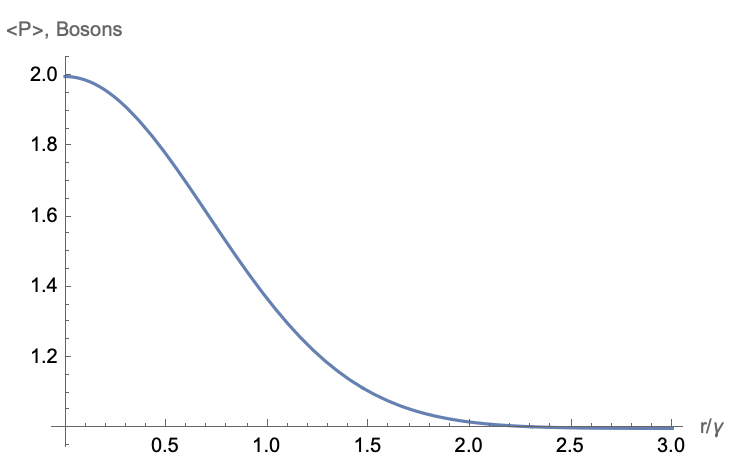
\includegraphics[width=0.8\textwidth]{figures/bosons_pic.png}
\caption{Bosons}
\end{minipage}
\begin{minipage}{0.4\textwidth}
\centering
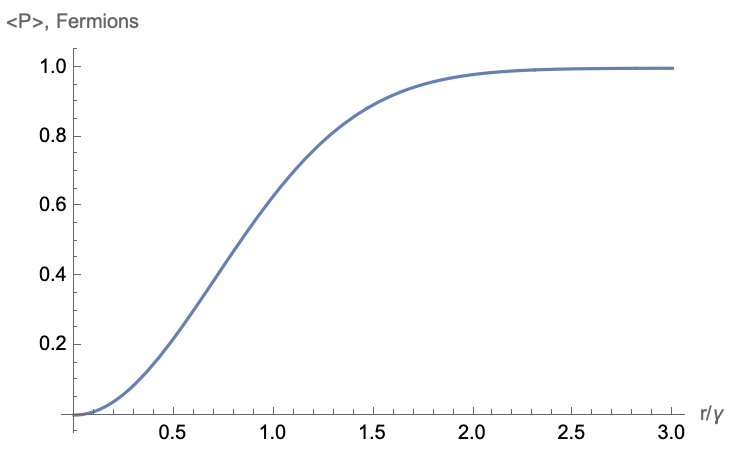
\includegraphics[width=0.8\textwidth]{figures/fermions_pic.png}
\caption{Fermions}
\end{minipage}
\end{figure*}



\item Assume that we have a pulse source of atoms with longitudinal dimension $L$. Atoms are released at time $t=0$ and are detected at time $t = \tau$.  Without loss of generality let's consider two atoms detected at the detector at the same time $t=\tau$. Let's also assume that the two atoms originate at the extreme ends of the sample (of length $L$).  Since the atoms arrive at the detector at the same time, the difference in momentum cannot exceed $mL/\tau$. From here, it is clear that
\begin{align*}
\hbar \vert{\vec{k}_l} \vert \leq \f{m L}{\tau}. 
\end{align*}
Now with $v = d/\tau$ being the velocity of the atoms, we find that
\begin{align*}
\vert (\vec{k}_A - \vec{k}_B)_l \vert \leq \f{mvL}{\hbar d}. 
\end{align*}
This implies that the different velocity groups separate during the expansion, narrowing (by a factor $L/d$)  velocity distribution of atoms detected at any particular time. \\

\noindent Assuming $L\approx W$ and $\tau = 0.1$ s, we can estimate the required timing resolution of the detector:
\begin{align*}
\tau \f{L}{d} = \tau \f{W}{d} = 56 \text{ \textmu s}.
\end{align*}
We can get this by argument by the extremes. If the sample is very small, then obviously we  want better timing resolution in order to resolve this longitudinal dimension of the atom sample. 


\end{itemize}

\item \textbf{Phase-space volume enhancement.} The peak in $g^{(2)}(1,2)$ is visible for $(\vec{k}_A - \vec{k}_B)\cdot \vec{r}_{21} \leq 2\pi$. This is equivalent to saying that we must detect atoms from within a single phase space cell, defined by $\delta p_x \delta x \leq h$. In our 3D atom sample, the 3D volume of a phase space cell is $\delta x \delta y \delta z = (\lambda_{dB})^3$. Liouville's theorem says that as our ball of atoms expands, the number of phase space cells remains constant. We now verify that the volume of a coherent phase space cell is increased by a factor $d^3 / W^2 L$ by the time the atoms reach the detector.\\

\noindent To see why this is true, we simply consider how a phase space cell evolves in volume as a function of time. Based on Part (c), we can see that the longitudinal dimension of the cell stretches by a factor $d/L$. Likewise, the transverse dimensions of the cell increase by $d/W$ each. Together, the total volume must increase by $d^3 / W^2 L$, as desired. \\

\noindent What is the order of magnitude of this increase? Assuming that $W\approx L \approx $ 56 \textmu m which is what we found in Part (a). Then increase factor is $(d/W)^3$ which is $(0.1 / 50 \times 10^{-6})^3$ which corresponds to roughly 9-10 orders of magnitude. \\

\noindent Here we estimate the average occupation of a cell of phase space for the $^6$Li MOT from parts (b) and (c). Assuming that there are $10^{10}$ atoms in $1$ cm$^3$. The volume of a phase space cell is $(\lambda_{dB})^3$ which corresponds to a volume of (31.8 nm)$^3$ for a $^6$Li MOT at 500 \textmu K. The average occupation is thus roughly $10^{-10}$. With the phase-space volume enhancement factor of $10^{10}$, the average occupation number is roughly unity, which is awesome. For comparison, the average occupation number of a BEC or a degenerate Fermi gas is also on the order of unity. 

\end{enumerate}





\end{document}








